% DO NOT COMPILE THIS FILE DIRECTLY!
% This is included by the other .tex files.

\begin{frame}[t,plain]
\titlepage
\end{frame}

\begin{frame}{Agenda}
    \input{../includes/agenda.txt}
\end{frame}

\begin{frame}
 \frametitle{MISP and starting from a practical use-case}
 \begin{itemize}
         \item During a malware analysis workgroup in 2012, we discovered that we worked on the analysis of the same malware.
         \item We wanted to share information in an easy and automated way {\bf to avoid duplication of work}.
         \item Christophe Vandeplas (then working at the CERT for the Belgian MoD) showed us his work on a platform that later became MISP.
         \item A first version of the MISP Platform was used by the MALWG and {\bf the increasing feedback of users} helped us to build an improved platform.
         \item MISP is now {\bf a community-driven development}.
 \end{itemize}
\end{frame}

\begin{frame}
\frametitle{about CIRCL}
The Computer Incident Response Center Luxembourg (CIRCL) is a government-driven initiative designed to provide a systematic response facility to computer security threats and incidents. CIRCL is the CERT for the private sector, communes and non-governmental entities in Luxembourg and is operated by securitymadein.lu g.i.e.
\end{frame}

\begin{frame}
\frametitle{MISP and CIRCL}
\begin{itemize}
\item CIRCL is mandated by the Ministry of Economy and acting as the Luxembourg National CERT for private sector.
\item CIRCL leads the development of the Open Source MISP threat intelligence platform which is used by many military or intelligence communities, private companies, financial sector, National CERTs and LEAs globally.
\item {\bf CIRCL runs multiple large MISP communities performing active daily threat-intelligence sharing}.
\end{itemize}
        
\includegraphics{en_cef.png}
\end{frame}


\begin{frame}
\frametitle{Development based on practical user feedback}
\begin{itemize}
\item There are many different types of users of an information sharing platform like MISP:
        \begin{itemize}
                \item {\bf Malware reversers} willing to share indicators of analysis with respective colleagues.
                \item {\bf Security analysts} searching, validating and using indicators in operational security.
                \item {\bf Intelligence analysts} gathering information about specific adversary groups.
                \item {\bf Law-enforcement} relying on indicators to support or bootstrap their DFIR cases.
                \item {\bf Risk analysis teams} willing to know about the new threats, likelyhood and occurences.
                \item {\bf Fraud analysts} willing to share financial indicators to detect financial frauds.
        \end{itemize}
\end{itemize}
\end{frame}

\begin{frame}
\frametitle{MISP model of governance}
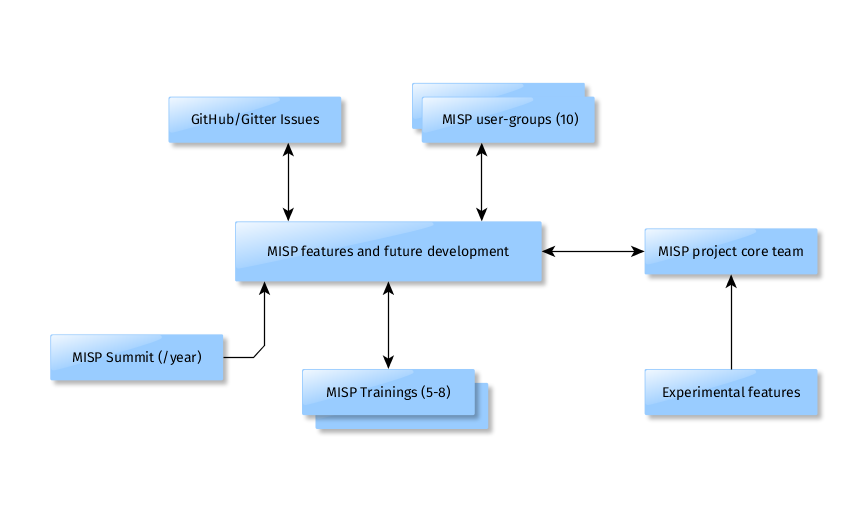
\includegraphics[scale=0.4]{governance.png}
\end{frame}

\begin{frame}
\frametitle{Many objectives from different user-groups}
        \begin{itemize}
                \item Sharing indicators for a {\bf detection} matter.
                        \begin{itemize}
                                \item 'Do I have infected systems in my infrastructure or the ones I operate?'
                        \end{itemize}
                \item Sharing indicators to {\bf block}.
                        \begin{itemize}
                                \item 'I use these attributes to block, sinkhole or divert traffic.'
                        \end{itemize}
                \item Sharing indicators to {\bf perform intelligence}.
                        \begin{itemize}
                                \item 'Gathering information about campaigns and attacks. Are they related? Who is targeting me? Who are the adversaries?'
                        \end{itemize}
                \item $\rightarrow$ These objectives can be conflicting (e.g. False-positives have different impacts)
        \end{itemize}
\end{frame}

\begin{frame}
\frametitle{Sharing Difficulties}
        \begin{itemize}
                \item Sharing difficulties are not really technical issues but often it's a matter of {\bf social interactions} (e.g. {\bf trust}).
                \item Legal restriction\footnote{\url{https://www.misp-project.org/compliance/}}
                        \begin{itemize}
                                \item "Our legal framework doesn't allow us to share information."
                                \item "Risk of information-leak is too high and it's too risky for our organization or partners."
                        \end{itemize}
                \item Practical restriction
                        \begin{itemize}
                                \item "We don't have information to share."
                                \item "We don't have time to process or contribute indicators."
                                \item "Our model of classification doesn't fit your model."
                                \item "Tools for sharing information are tied to a specific format, we use a different one."
                        \end{itemize}
        \end{itemize}
\end{frame}


\begin{frame}
        \frametitle{MISP Project Overview}
        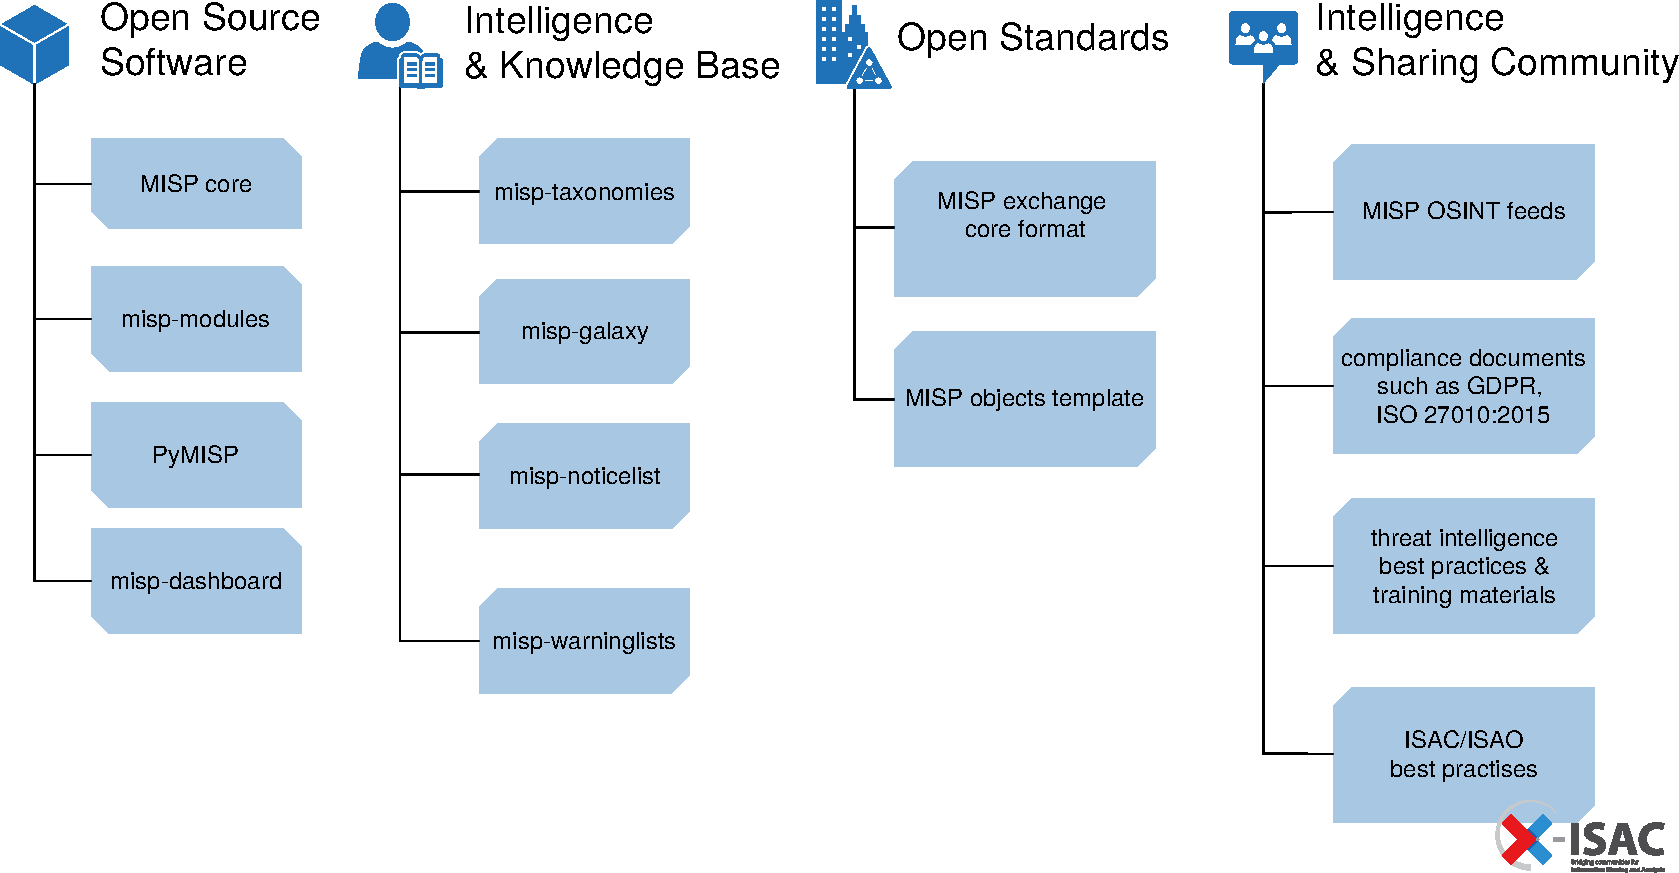
\includegraphics[scale=0.35]{misp-overview-simplified.pdf}
\end{frame}

%\begin{frame}
%        \frametitle{MISP Project Overview}
%        \begin{columns}[t]
%        \column{5.0cm}
%        \begin{figure}
%        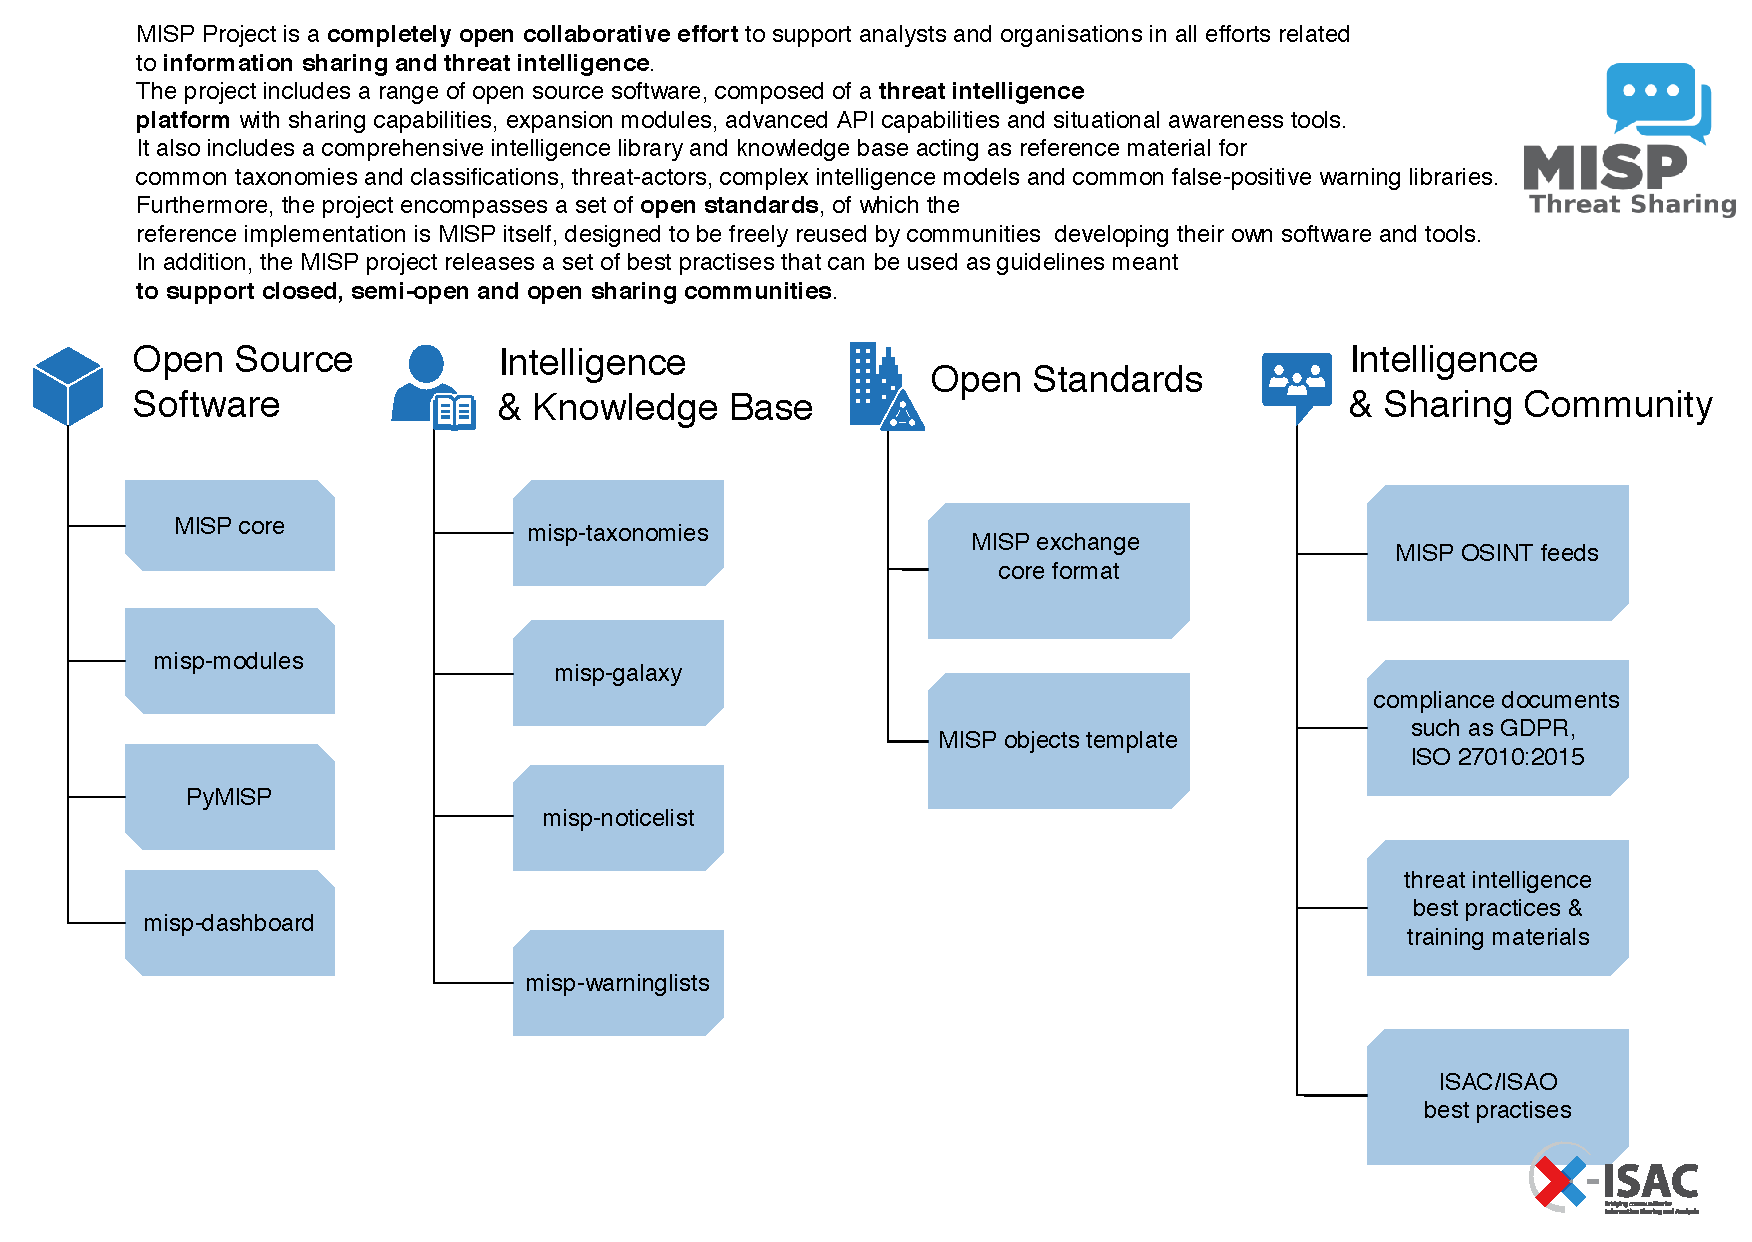
\includegraphics[scale=0.20]{misp-overview.pdf}\\
%        \end{figure}
%        \column{7cm}
%        \begin{itemize}
%                \item The {\bf core project}\footnote{\url{http://github.com/MISP/}} (PHP/Python3) supports the backend, API \& UI.
%                \item Modules (Python3) expand MISP functionalities.
%                \item Taxonomies (JSON) to add categories \& global tagging.
%                \item Warning-lists (JSON) help analysts to detect potential false-positives.
%                \item Galaxy (JSON) to add threat-actors, tools or "intelligence".
%                \item Objects (JSON) to allow for templated composition of security related atomic points of information.
%        \end{itemize}
%        \end{columns}
%\end{frame}

\begin{frame}
 \frametitle{MISP features}
 \begin{itemize}
         \item MISP\footnote{\url{https://github.com/MISP/MISP}} is a threat information sharing free \& open source software.
         \item MISP has {\bf a host of functionalities} that assist users in creating, collaborating \& sharing threat information - e.g. flexible sharing groups, {\bf automatic correlation}, free-text import helper, event distribution \& proposals.
         \item Many export formats which support IDSes / IPSes (e.g. Suricata, Bro, Snort), SIEMs (eg CEF), Host scanners (e.g. OpenIOC, STIX, CSV, yara), analysis tools (e.g. Maltego), DNS policies (e.g. RPZ).
         \item A rich set of MISP modules\footnote{\url{https://www.github.com/MISP/misp-modules}} to add expansion, import and export functionalities.
 \end{itemize}
\end{frame}

\begin{frame}
        \frametitle{Correlation features: a tool for analysts}
        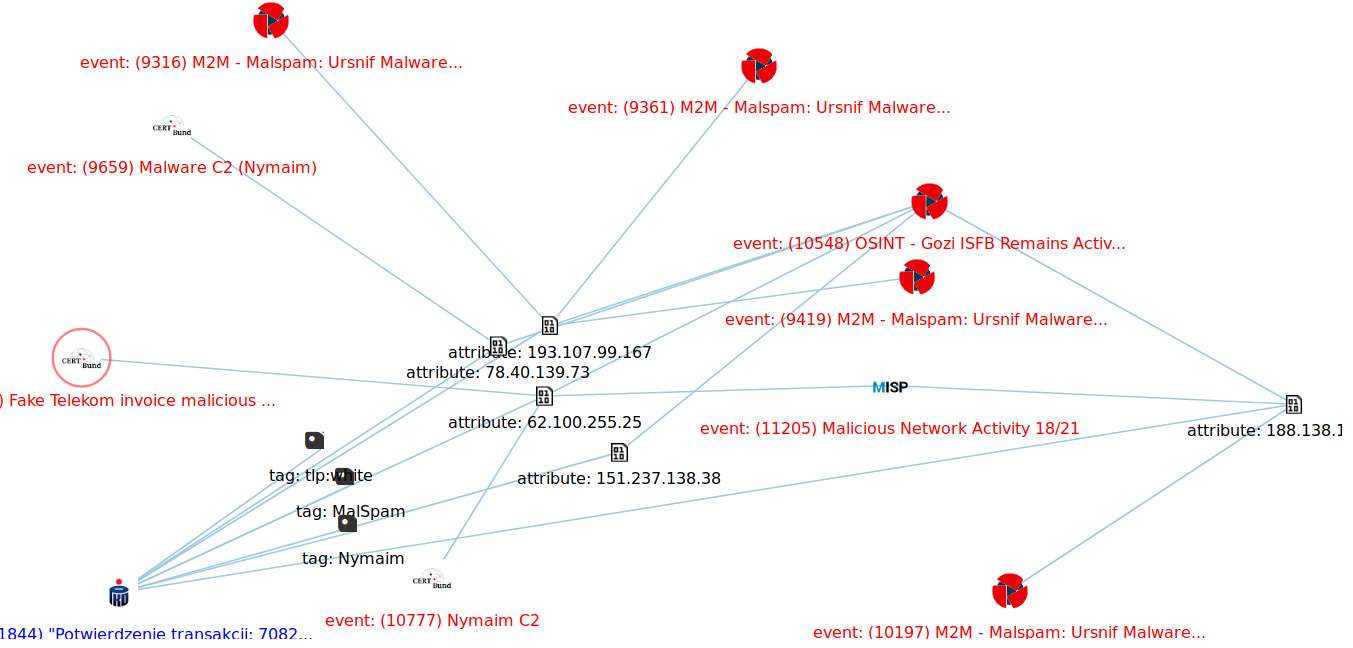
\includegraphics[scale=0.18]{screenshots/campaign.png}
        \begin{itemize}
                \item To {\bf corroborate a finding} (e.g. is this the same campaign?), {\bf reinforce an analysis} (e.g. do other analysts have the same hypothesis?), {\bf confirm a specific aspect} (e.g. are the sinkhole IP addresses used for one campaign?) or just find if this {\bf threat is new or unknown in your community}.
        \end{itemize}
\end{frame}


\begin{frame}
 \frametitle{Communities using MISP}
 \begin{itemize}
	 \item Communities are groups of users sharing within a set of common objectives/values.
	 \item CIRCL operates multiple MISP instances with a significant user base (more than 950 organizations with more than 2400 users).
     \item {\bf Trusted groups} running MISP communities in island mode (air gapped system) or partially connected mode.
	 \item {\bf Financial sector} (banks, ISACs, payment processing organizations) use MISP as a sharing mechanism.
	 \item {\bf Military and international organizations} (NATO, military CSIRTs, n/g CERTs,...).
	 \item {\bf Security vendors} running their own communities (e.g. Fidelis) or interfacing with MISP communities (e.g. OTX).
 \end{itemize}
\end{frame}


\begin{frame}
\frametitle{MISP core distributed sharing functionality}
\begin{itemize}
\item MISPs' core functionality is sharing where everyone can be a consumer and/or a contributor/producer."
\item Quick benefit without the obligation to contribute.
\item Low barrier access to get acquainted to the system.
\end{itemize}
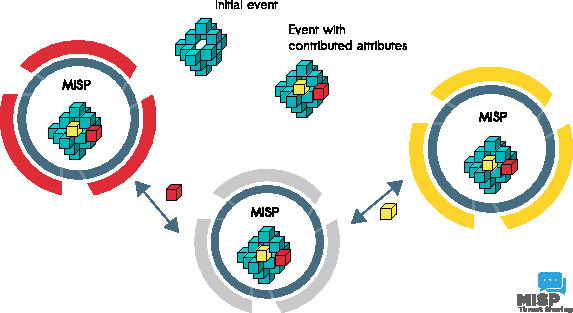
\includegraphics[scale=0.9]{misp-distributed.pdf}
\end{frame}


\begin{frame}
        \frametitle{Events, Objects and Attributes in MISP}
         \begin{itemize}
                \item MISP events are encapsulations for contextually linked information
                \item MISP attributes\footnote{attributes can be anything that helps describe the intent of the event package from indicators, vulnerabilities or any relevant information} initially started with a standard set of "cyber security" indicators.
                \item MISP attributes are purely {\bf based on usage} (what people and organizations use daily).
                \item Evolution of MISP attributes is based on practical usage \& users (e.g. the addition of {\bf financial indicators} in 2.4).
                \item MISP objects are attribute compositions describing points of data using many facets, constructed along the lines of community and user defined templates.
                \item Galaxies granularly contextualise, classify \& categorise data based on {\bf threat actors}, {\bf preventive measures}, tools used by adversaries.
        \end{itemize}
\end{frame}
\begin{frame}
        \frametitle{Terminology about Indicators}
        \begin{itemize}
                \item Indicators\footnote{IoC (Indicator of Compromise) is a subset of indicators}
                        \begin{itemize}
                                \item Indicators contain a pattern that can be used to detect suspicious or malicious cyber activity.
                        \end{itemize}
                \item Attributes in MISP can be network indicators (e.g. IP address), system indicators (e.g. a string in memory) or even bank account details.
                \begin{itemize}
                        \item {\bf A type (e.g. MD5, url) is how an attribute is described}.
                \end{itemize}
                \begin{itemize}
                \item An attribute is always in a category (e.g. Payload delivery) which puts it in a context.
                        \begin{itemize}
                                \item {\bf A category is what describes} an attribute.
                        \end{itemize}
                \item An IDS flag on an attribute allows to determine if {\bf an attribute can be automatically used for detection}.
                \end{itemize}
        \end{itemize}
\end{frame}


\begin{frame}
        \frametitle{Sharing Attackers Techniques}
        \begin{itemize}
                \item MISP integrates at event or attribute level MITRE's Adversarial Tactics, Techniques, and Common Knowledge (ATT\&CK).
        \end{itemize}
        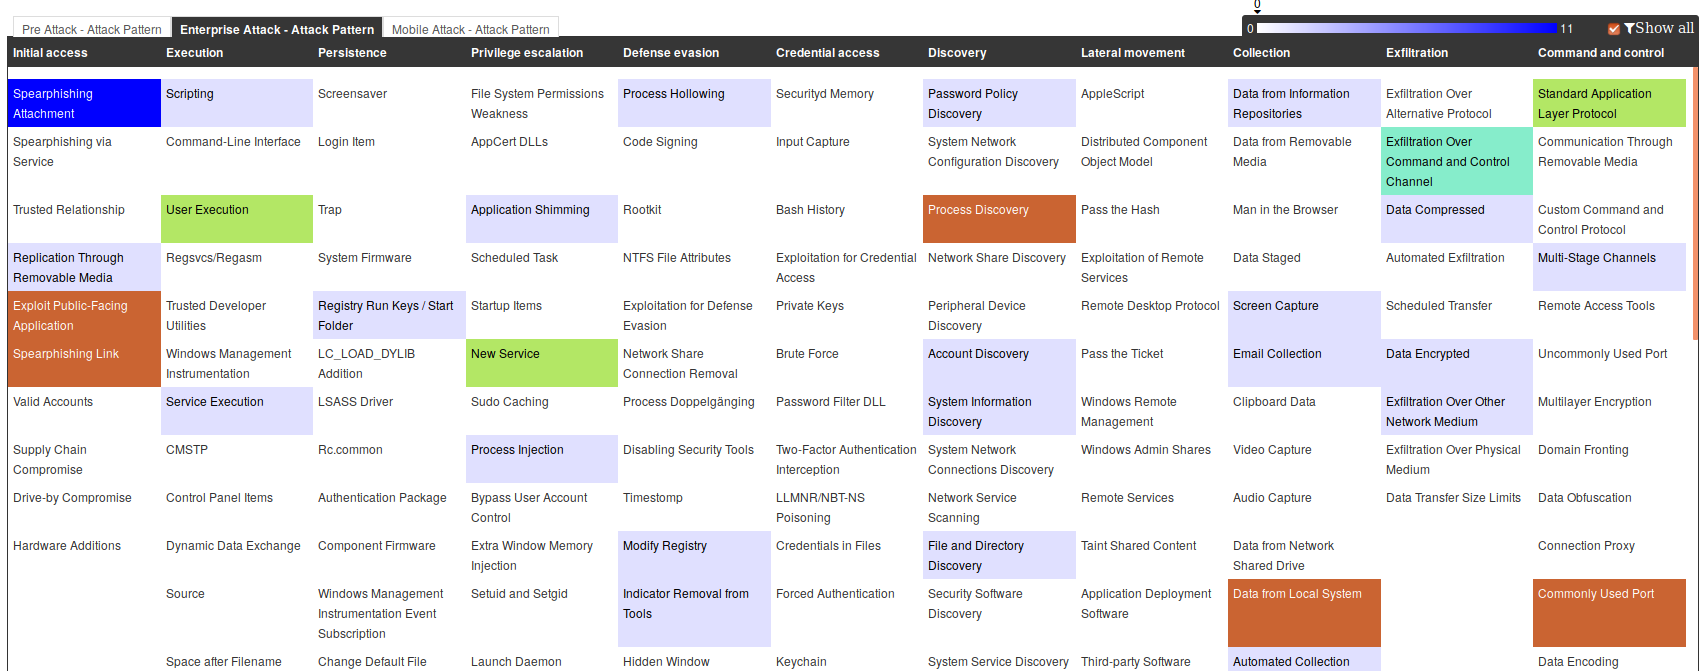
\includegraphics[scale=0.2]{screenshots/attack-screenshot.png}
\end{frame}

\begin{frame}
        \frametitle{Supporting specific datamodel}
        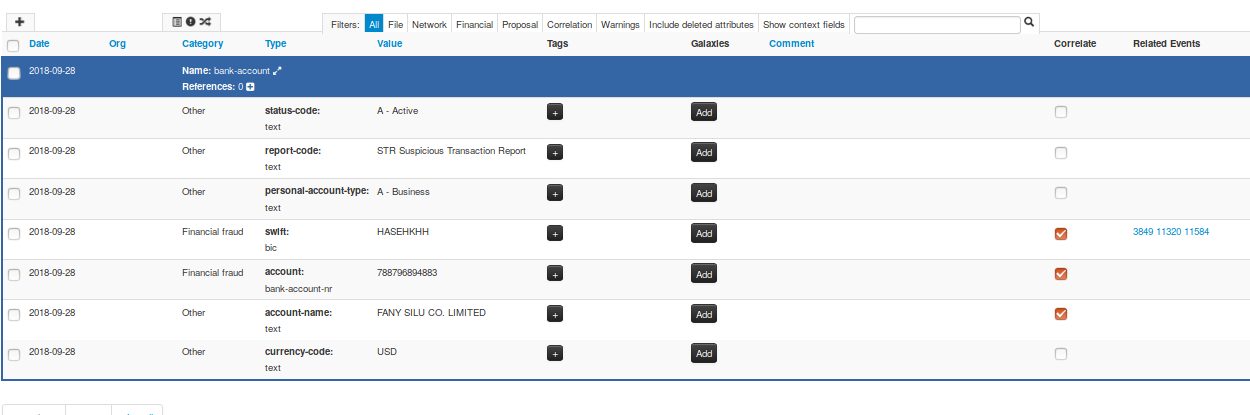
\includegraphics[scale=0.24]{screenshots/bankaccount.png}
        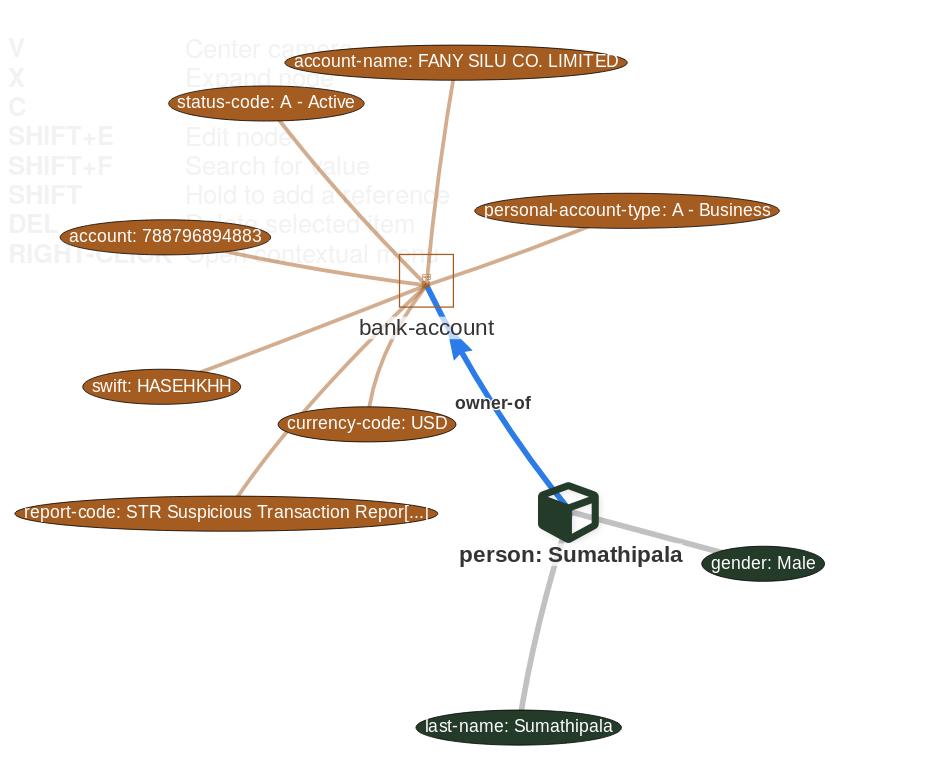
\includegraphics[scale=0.18]{screenshots/bankview.png}
\end{frame}

\begin{frame}
        \frametitle{Helping Contributors in MISP}
        \begin{itemize}
            \item Contributors can use the UI, API or using the freetext import to add events and attributes.
                \begin{itemize}
                        \item Modules existing in Viper (a binary framework for malware reverser) to populate and use MISP from the vty or via your IDA.
                \end{itemize}
        \item Contribution can be direct by creating an event but {\bf users can propose attributes updates} to the event owner.
            \item {\bf Users should not be forced to use a single interface to contribute}.
        \end{itemize}
\end{frame}

\begin{frame}
        \frametitle{Example: Freetext import in MISP}
        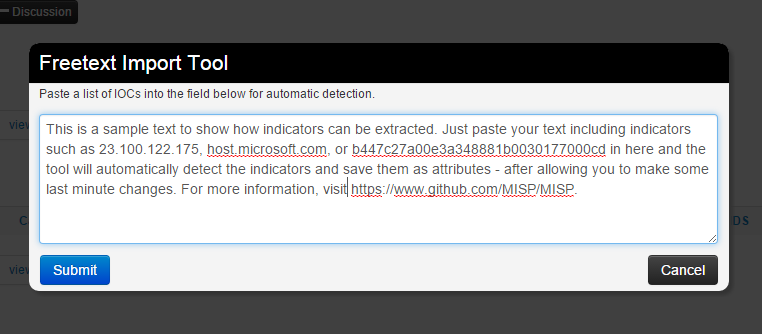
\includegraphics[scale=0.3]{screenshots/freetext1.PNG}\\
        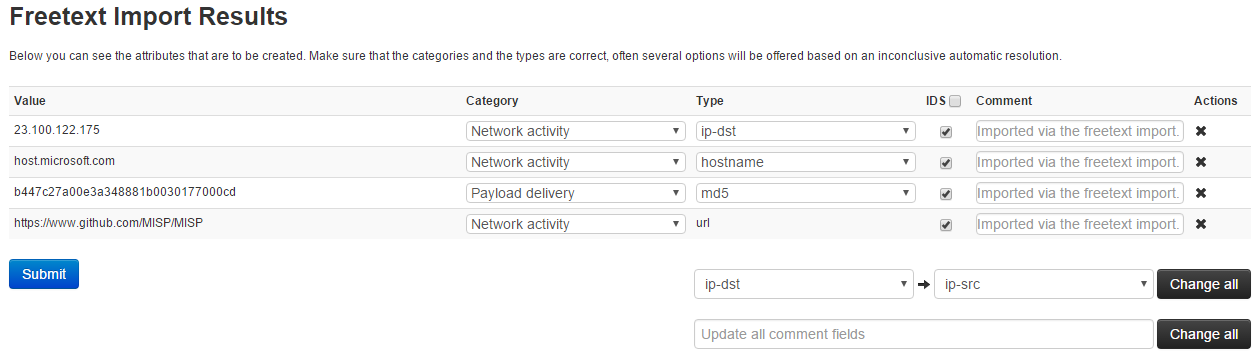
\includegraphics[scale=0.3]{screenshots/freetxt2.PNG}\\
        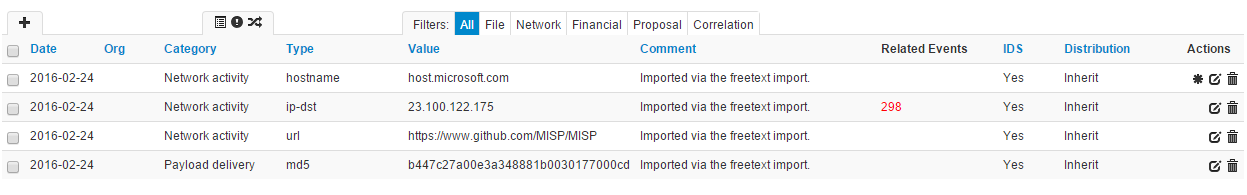
\includegraphics[scale=0.3]{screenshots/freetxt3.PNG}
\end{frame}

\begin{frame}
        \frametitle{Supporting Classification}
        \begin{itemize}
          \item Tagging is a simple way to attach a classification to an event or an attribute.
          \item {\bf Classification must be globally used to be efficient}.
          \item MISP includes a flexible tagging scheme where users can select from more than 42 existing taxonomies or create their own taxonomy.
        \end{itemize}
        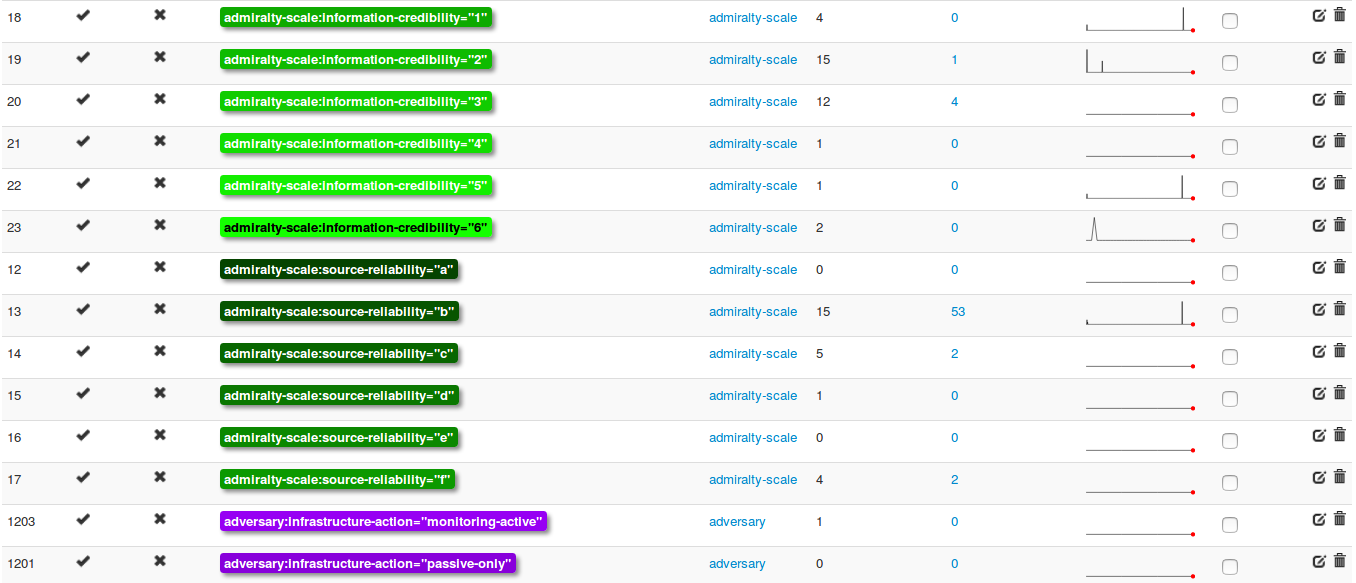
\includegraphics[scale=0.20]{tags-2-4-70.png}
\end{frame}

\begin{frame}
\frametitle{Supporting Sharing in MISP}
\begin{itemize}
        \item Delegate events publication to another organization (introduced in MISP 2.4.18).
        \begin{itemize}
                \item The other organization can take over the ownership of an event and provide {\bf pseudo-anonymity to initial organization}.
        \end{itemize}
        \item Sharing groups allow custom sharing (introduced in MISP 2.4) per event or even at attribute level.
        \begin{itemize}
                \item Sharing communities can be used locally or even cross MISP instances.
                \item {\bf Sharing groups} can be done at {\bf event level or attributes level} (e.g. financial indicators shared to a financial sharing groups and cyber security indicators to CSIRT community).
        \end{itemize}
\end{itemize}
\end{frame}

\begin{frame}
        \frametitle{Sightings support}
        \begin{columns}[t]
        \column{5.0cm}
        \begin{figure}
        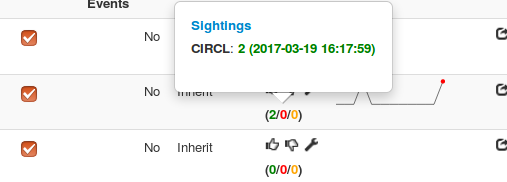
\includegraphics[scale=0.3]{screenshots/sighting-n.png}\\
        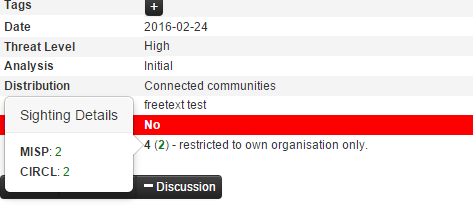
\includegraphics[scale=0.34]{screenshots/Sightings2.PNG}
        \end{figure}
        \column{7cm}
        \begin{itemize}
                \item Sightings allow users to notify the community about the activities related to an indicator.
                \item In recent MISP versions, the sighting system supports negative sigthings (FP) and expiration sightings.
                \item Sightings can be performed via the API, and the UI, even including the import of STIX sighting documents.
                \item Many use-cases for scoring indicators based on users sighting.
        \end{itemize}
        \end{columns}
\end{frame}


\begin{frame}
\frametitle{Improving Information Sharing in MISP}
\begin{itemize}
        \item False-positives are a recurring challenge in information sharing.
        \item In MISP 2.4.39, we introduced the misp-warninglists\footnote{\url{https://github.com/MISP/misp-warninglists}} to help analysts in their day-to-day job.
        \item Predefined lists of well-known indicators which are often false-positives like RFC1918 networks, public DNS resolver are included by default.
\end{itemize}
\end{frame}

\begin{frame}
\frametitle{Improving support of sharing within and outside an organization}
\begin{itemize}
        \item Even in a single organization, multiple use-cases of MISP can appear (groups using it for dynamic malware analysis correlations, dispatching notification).
        \item In MISP 2.4.51, we introduced the ability to have {\bf local MISP} servers connectivity to avoid changes in distribution level. This allows to have mixed synchronization setup within and outside an organization.
        \item Feed support was also introduced to support synchronization between untrusted and trusted networks.
\end{itemize}
\end{frame}

\begin{frame}
        \frametitle{Bootstrapping MISP with indicators}
        \begin{itemize}
                \item We maintain the default CIRCL OSINT feeds (TLP:WHITE selected from our communities) in MISP to allow users to ease their bootstrapping.
                \item The format of the OSINT feed is based on standard MISP JSON output pulled from a remote TLS/HTTP server.
                \item Additional content providers can provide their own MISP feeds. (\url{https://botvrij.eu/})
                \item Allows users to {\bf test their MISP installations and synchronisation with a real dataset}.
                \item Opening contribution to other threat intel feeds but also allowing the analysis of overlapping data\footnote{A recurring challenge in information sharing}.
        \end{itemize}
\end{frame}


\begin{frame}
        \frametitle{Conclusion}
        \begin{itemize}
                \item {\bf Information sharing practices come from usage} and by example (e.g. learning by imitation from the shared information).
                \item MISP is just a tool. What matters is your sharing practices. The tool should be as transparent as possible to support you.
                \item Enable users to customize MISP to meet their community's use-cases.
                \item MISP project combines open source software, open standards, best practices and communities to make information sharing a reality.
        \end{itemize}
\end{frame}

\begin{frame}{MISP User Experience Survey}

  A researcher--Borce STOJKOVSKI--from University of Luxembourg (SnT) is
  conducting a survey about MISP UX.
  \vspace{1cm}
  \begin{itemize}
    \item You may participate at the following location: \url{https://misp-project.org/ux-survey}
    \item on-voluntary basis: opt-out at any time,
    \item results will be communicated back to the community and used to improve
      MISP's User Interface,
    \item for any inquiries contact ux@misp-project.org
  \end{itemize}
  

\end{frame}

